\documentclass[english, 11pt]{article}
\usepackage{../notes}

\newcommand{\thiscoursecode}{PHYS 234}
\newcommand{\thiscoursename}{Quantum Physics I}
\newcommand{\thisprof}{Dr. Robert Hill}
\newcommand{\me}{Liam Horne}
\newcommand{\thisterm}{Spring 2014}
\newcommand{\website}{LIHORNE.COM}

% Headers
\lhead{\thisterm}

%%%%% TITLE %%%%%
\newcommand{\notefront} {
\pagenumbering{roman}
\begin{center}

{\ttfamily \url{\website}} {\small}

\textbf{\Huge{\noun{\thiscoursecode}}}{\Huge \par}

{\Large{\noun{\thiscoursename}}}\\ \vspace{0.1in}

\vspace{0in}
\includegraphics[scale=0.5]{../logo.png}

  %\includegraphics[scale=0.1]{shield.png} \\
  {\noun \thisprof} \ $\bullet$ \ {\noun \thisterm} \ $\bullet$ \ {\noun {University of Waterloo}} \\

  \end{center}
  }

%   ooooo      ooo   .oooooo.   ooooooooooooo oooooooooooo  .oooooo..o
%   `888b.     `8'  d8P'  `Y8b  8'   888   `8 `888'     `8 d8P'    `Y8
%    8 `88b.    8  888      888      888       888         Y88bo.
%    8   `88b.  8  888      888      888       888oooo8     `"Y8888o.
%    8     `88b.8  888      888      888       888    "         `"Y88b
%    8       `888  `88b    d88'      888       888       o oo     .d8P
%   o8o        `8   `Y8bood8P'      o888o     o888ooooood8 8""88888P'

\begin{document}

  % Notes fron
  \notefront
  % Table of Contents and List of Figures
  \tocandfigures
  % Abstract
  \doabstract{These notes are intended as a resource for myself; past, present, or future students of this course, and anyone interested in the material. The goal is to provide an end-to-end resource that covers all material discussed in the course displayed in an organized manner. If you spot any errors or would like to contribute, please contact me directly. \\}

  Robert Hill is a low temperature experimentalist, but this course will be mostly theoretical.
  \newline

   Albert Einstein once said, "Quantum mechanics is certainly imposing. But an inner voice tells me that it is not yet the realthing. The theory says a lot, but does not really bring us any closer to the secret of the 'old one'. I, at any rate, am convinced that He does not throw dice."
   \newline

   Richard Feynman said "I think I can safely say that nobody understand quantum mechanics."
   \newline

   So we're in for miserable experience with this course then? Well not really, there are some good reasons to study Quantum Physics:

   \begin{itemize}
     \item It's Extremely interesting!
     \begin{itemize}
        \item Physically
        \item Mathematically
        \item Philosophically
      \end{itemize}
      \item It is the science behind future technology!
      \item Waterloo is Quantum Valley!
   \end{itemize}

   \section{The Photoelectric and Compton Effects}

     \subsection{Historical Background}
       In classical physics we always observed things as behaving like waves or as particles. For example, there is

       \begin{itemize}
         \item Particle-like behaviour of radiation
         \item Wave-like behaviour of matter
         \item Wave-particle duality that combines the two
       \end{itemize}

       Let's explore the two sides of the coin. First, {\bf what is a particle?} Some words that describe it are {\textit point, localised, mass, solid} and similarly {\bf what is a wave?} It can be described with words like \textit{interference, oscillation, delocalised}, and \textit{medium}. One such thing that we have had trouble with describing is {\bf light}. Is it a wave or a particle?

     \subsection{Einstein's Theory of Photoelectric Effect}

       Radiant energy (light) is quantized into concentrated bundles (photons)

       \[ E = hf \]

       His Photoelectric Equation (1905) states that

       \[ K_{\mbox{max}} = hf - \omega_0 \]

     \subsection{Compton Effect}

       In the photoelectric effect, we treated light as being composed of individual light particles, called photons, that carry some energy. It then makes sense to think that the photons also have momentum.
       \newline

       Electromagnetic radiation is scattered by a target object. In classical theory, the charges in the target object will respond to the incoming wave and start to oscillate. All oscillating charges emit radiation at the frequency of oscillation, and this newly generated set of waves can also be detected at an angle θ with respect to the incoming wave. This classical model explains why the sky is blue and all that jazz. The scattering process itself, though, does not change the frequency of incoming and outgoing radiation.
       \newline

       However, an experimental problem occurred. In experiments with X-ray radiation on a graphene target, one observes that two separate frequencies at an angle $\theta$ result in different intensities. This effect is independent of the material, though intensities may vary.
       \newline

       \begin{defn}[Compton Shift]\label{compton_shift}
         \[ \Delta \lambda = \lambda_c (1 - \cos \theta) \]
       \end{defn}

       \begin{defn}[Compton wavelength]\label{compton_wavelength}
         \[ \lambda_c = \f{h}{m_0c} \]
       \end{defn}

       \begin{figure}[t]
         \centering
           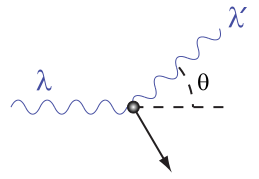
\includegraphics[width=0.35\textwidth]{compton_scattering.png}
         \caption{The Compton Effect. The scattered light has a different frequency; the frequency depends on the direction. A bigger deflection causes a bigger change in frequency.}
       \end{figure}

   \section{De Broglie Wavelength and the Davisson-Germer Experiement}

     We have shown that wave phenomena can exhibit particle features. We can rewrite the momentum instead as $p = \f{h}{\lambda}$ using a simple wave relationship. There is nothing in this reformed equation that has to do with light. This led to the following postulate.

     \subsection{The De Broglie Postulate (1924)}
       De Broglie's hypothesis was based on the grand symmetry of nature; if radiation has wave-particle duality, then so should matter.
       \begin{defn}[de Broglie Relation]\label{de_broglie_relation}
         \[ \lambda = \f{h}{p} \]
       \end{defn}

     \subsection{The Davisson-Germer Experiment}
       We must first understand the Bragg Grating; it is an optical filter that reflects particular wavelengths and transmits all others. Note that reflection, however, is common to both waves and particles.

     \subsection{Final Words}
       The observation of both phenomena in one and the same experiment leads us also to the concept of delocalization, which goes beyond the simple concept of "being extended", because single quantum objects seem to be able to simultaneously explore regions in space-time that cannot be explored by a single object in any classical way.

   \section{Linear Algebra Review}

     We're going to begin by reviewing some mathematics that will be needed in the course. This is a physics course so we're going to be a little loosey-goosey.

     \subsection{Vector Spaces}
        \begin{defn}[Vector Space]\label{vector_space}
          A {\bf vector space} consists of a set of vectors : ($|\alpha\rangle, |\beta\rangle, |\gamma\rangle, \ldots$) which is closed under vector addition and scalar multiplication.
        \end{defn}
        {\bf Vector Addition} produces another vector, that is
        \[ \ket{\alpha} + \ket{\beta} = \ket{\gamma}  \]
        it is also commutative
        \[ \ket{\alpha} + \ket{\beta} =  \ket{\beta}  + \ket{\alpha} \]
        and associative
        \[ \ket{\alpha} + (\ket{\beta} + \ket{\gamma}) =  (\ket{\alpha}+\ket{\beta} ) + \ket{\gamma} \]
        The null vector exists such that $\ket{\alpha} + \ket{0} = \ket{\alpha}$, and of course there is the inverse vector such that $\ket{\alpha} + \ket{-\alpha} = \ket{0}$.
        \newline

        {\bf Scalar Multiplication}: The product of a scalar with a vector is another vector ($a\ket{\alpha} = \ket{\gamma}$). Note that scalar multiplication is distributive with respect to vector addition
        \[ a(\ket{\alpha} + \ket{\beta}) = a\ket{\alpha} + a\ket{\beta} \]
        Scalar multiplication is distributive with respect to scalar addition too
        \[ (a + b)\ket{\alpha} = a\ket{\alpha} + b\ket{\alpha} \]
        and it is associative with respect to the product of scalars.
        \[ a(b \ket{\alpha}) = (ab)\ket{\alpha} \]
        then multiplication by zero and by $\pm 1$ has
        \[ 0\ket{\alpha} = \ket{0}, \ \ \ \ 1\ket{\alpha} = \ket{\alpha}, \ \ \ \ -1\ket{\alpha} = -\ket{\alpha} = \ket{-\alpha} \]
        \newline

        {\bf Linear Combinations of Vectors}: To generate a linear combination of vectors
        \[ \ket{\lambda} = a\ka + b\kb + c\kg \]
        \begin{itemize}
          \item[(I)] Any vector is linearly independent of a set of vectors if it cannot be written as a linear combination of them.
          \item[(II)] A set of vectors is linearly independent if each is linearly independent of the rest.
          \item[(III)] A colelction of vectors is said to {\bf span} the space if every vector can be written as a linear combination of them.
          \item[(IV)] A set of linearly independent vectors that span a space is called a {\bf basis}.
          \item[(V)] The number of vectors in the basis is called the {\bf dimension} of the space.\newline
        \end{itemize}

        {\bf Co-ordinate Representation}: With respect to a given basis, $\ket{e_1}, \ket{e_2}, \ket{e_3}, \hdots, \ket{e_n}$, any given vector $\ka = a_1 \ket{e_1} + a_2\ket{e_2} + \hdots + a_n \ket{e_n}$ is uniquely defined by the ordered $n$-tuple of its components.
        \[ \ka \iff \left(\begin{matrix}a_1 \\ a_2 \\ \vdots \\ a_n\end{matrix}\right) \]
        (the co-ordinate representation of $\ka$ with respect to the basis given by each $\ket{e_1}$.)

        Coordinates depend on the chosen basis. In basis 1 $\ka = a_x\ket{x} + a_y\ket{y} \iff \left(\begin{matrix}a_x \\ a_y \end{matrix}\right)$ and then in basis 2 we see $\ka = a_{x'}\ket{x'} + a_{y'}\ket{y'} \iff \mtx{a_{x'} \\ a_{y'}}$. \newline

        Addition of vectors by adding corresponding components (when in the same basis) works as you might expect, too:
        \[ \ket{\alpha} + \ket{\beta} \iff (a_1 + b_1, a_2 + b_2, \hdots, a_n + b_n \]

        Also, scalar multiplication works by multiplying the scalar in each component
        \[ c\ka \iff (ca_1, ca_2, ca_3, \ldots, ca_n) \]
        so of course,
        \[ \ket{0} = (0, 0, 0, \ldots, 0),  \ \ \ \ \ \ \  \ket{-\alpha} = (-a_1, -a_2, \ldots, -a_n) \]

        {\bf Inner Product}: For every vector, $\ka$, in a vector space there exists a dual vector $\bra{\alpha}$ in a corresponding dual vector space. Importantly, the dual vector to $c\ka$ is $C^*\bra{\alpha}$ where $*$ denotes complex conjugation. So the inner product of $\ka$ and $\kb$ is $\braket{\alpha}{\beta}$ which is a scalar (complex number), hence $\braket{\alpha}{\beta}$ is sometimes called {\bf scalar product}.

        \begin{itemize}
          \item[(I)] $\braket{\beta}{\alpha} = \braket{\alpha}{\beta}^*$
          \item[(II)] $\braket{\alpha}{\alpha} \geq 0$ (real and positive), so $\braket{\alpha}{\alpha} = 0$ if $\ka = \ket{0}$.
          \item[(III)] The norm of a vector $||\alpha|| = \sqrt{\braket{\alpha}{\alpha}}$ generalized "length" of a vector.
          \item[(IV)] Normalized $||\alpha|| = 1$.
          \item[(V)] Orthogonal if $\braket{\alpha}{\beta} = 0$, then $\ka$ is orthogonal to $\kb$.
          \item[(VI)] Orthogonal set $\braket{a_i}{a_j} = \delta_{ij} = \piecewise{1}{if $i = j$}{0}{if $i \not = j$}$
        \end{itemize}

        Consider the orthonormal basis $\ebasis$, and
        \[ \ka = a_1 \ket{e_1} + a_2 \ket{e_2} + \ldots + a_n \ket{e_n} \]
        \[ \kb = b_1 \ket{e_1} + b_2 \ket{e_2} + \ldots + b_n \ket{e_n} \]
        where we have the column vectors
        \[ \ka = \mtx{a_1 \\ a_2 \\ \vdots \\ a_n} \ \ \ \ \ \ \ \ \kb = \mtx{b_1 \\ b_2 \\ \vdots \\ b_n} \]
        then with dual vectors
        \[ \ka  = a_1^*\ket{e_1} + a_2^*\ket{e_2} + \ldots + a_n^*\ket{e_n} \]
        \[ \kb  = b_1^*\ket{e_1} + b_2^*\ket{e_2} + \ldots + b_n^*\ket{e_n} \]
        so that we have row vectors
        \[ \ka = (a_1^*, a_2^*, \ldots, a_n^*)  \ \ \ \ \ \ \ \ \kb = (b_1^*, b_2^*, \ldots,b_n^*) \]
        Now we can see that these results interact in a kind of cool way, check this out:
        \[ \braket{\alpha}{\beta} = (a_1^*, a_2^*, \ldots, a_n^*) \mtx{b_1 \\ b_2 \\ \vdots \\ b_n} = a_1^*b_1 + a_2^*b_2 + \ldots + a_n^* b_n \]
        which is a complex number. The components of the linear expansion are inner products too:
        \[ \ka = a_1\ket{e_1} + a_2\ket{e_2} + \ldots + a_n\ket{e_n} \]
        Consider also that
        \[ \braket{e_1}{\alpha} = \braket{e_1}{\left(a_1\ket{e_1} + a_2\ket{e_2} + \ldots + a_n\ket{e_n}\right)} = a_1\braket{e_1}{e_1} + a_2\braket{e_1}{e_2} + \ldots + a_n\braket{e_1}{e_n} = a_1\]

     \subsection{Matrices}

        Matrices represent linear transformations that take a vector in a vector space and map it to another vector.
        \[ \ket{\alpha} \longrightarrow \ket{\alpha'}= \hat{T} \ket{\alpha} \]
        The transformation must be linear
        \[ \hat{T}(a \ket{\alpha} + b \ket{\beta}) = a\hat{T}\ket{\alpha} + b \hat{T}\ket{\beta} \]
        Consider $\hat{T}$ acting on $n$ basic vectors, $\ket{e_i}$
        \[ \hat{T} \ket{e_1} = T_{11}\ket{e_1} + T_{21}\ket{e_2} + \ldots + T_{n1} \ket{e_n} \]
        That is, $\ket{e_1}$ is mapped to a new vector written as a linear combination of basis vectors, likewise
        \begin{align*}
          \hat{T} \ket{e_2} & = T_{12}\ket{e_1} + T_{22}\ket{e_2} + \ldots + T_{n2} \ket{e_n} \\
          & \vdots \\
          \hat{T} \ket{e_n} & = T_{1n} \ket{e_1} + T_{2n} \ket{e_2} + \ldots + T_{nn} \ket{e_n}
        \end{align*}
        which can be compactly expressed
        \[ \hat{T}\ket{e_j} = \sum_{i=1}^nT_{ij} \ket{e_i} \ \ \ \ \ \ (j = 1,2,\ldots,n) \]
        If $\ket{\alpha}$ is an arbitrary vector, expressed in terms of basis $\ket{e_i}$'s
        \[ \ket{\alpha} = a_1\ket{e_1} + a_2\ket{e_2} + \ldots + a_n\ket{e_n} = \sum_{j=1}^n a_j\ket{e_j} \]
        (and recall $a_i = \braket{e_1}{\alpha}$). Then the effect of $\hat{T}$ on $\ka$ is
        \[ \hat{T}\ka = \sum_{j=1}^n a_j \hat{T} \ket{e_j} = \sum_{j=1}^n \sum_{i=1}^n a_j T_{ij} \ket{e_i} = \sum_{i=1}^n \left( \sum_{j=1}^n T_{ij}a_j \right) \ket{e_i} \]
        Hence $\hat{T}$ takes a vector $\ka$, with components $a_1, a_2, \ldots, a_n$ and maps to a new vector $\alpha'$ with components $a_i' = \sum_{j=1}^n T_{ij} a_j$. So $\hat{T}$ is characterized by $n^2$ elements, $T_{ij}$, which depend on the chosen basis. Express $\hat{T}$ as a matrix.
        \[ \mtx{T_{11} & T_{12} & \hdots & T_{1n} \\ T_{21} & T_{22} & \hdots & T_{2n} \\ \vdots & \ddots & \ddots & \vdots \\ T_{n1} & T_{n2} & \hdots & T_{nn} } \]
        where $T_{ij}$ is a matrix element, the row is $i$ and column $j$. Now if we want to express $\hat{T}$ with respect to a particular set of basis vectors, the $i$-th element will define the values of matrix elements $T_{ij}$
        \[ \hat{T}\ket{e_j} = \sum_{i=1}^n \ket{e_i} \ \ \ \ \ (j = 1,2,\ldots,n) \]
        multiply on left by basis vector $\ket{e_k}$,
        \begin{align*}
          \bra{e_k}\hat{T}\ket{e_j} & = \bra{e_k}\sum_{i = 1}T_{ij}\ket{e_i} \\
          & = \bra{e_k} \left(T_{ij}\ket{e_1} + T_{2j}\ket{e_2} + \ldots + T_{nj} \ket{e_n} \right) \\
          & = \left( T_{ij} = \braket{e_k}{e_1} + T_{2j}\braket{e_k}{e_2} + \ldots + T_{kj}\braket{e_k}{e_k} + \ldots + T_{nj}\braket{e_k}{e_n} \right)
        \end{align*}
        where all terms except $\braket{e_k}{e_k}$ go to 0. Now apply the orthonormal property of basis vectors $\ket{e_i}$ and thus
        \[ \bra{e_k}\hat{T}\ket{e_j} = T_{kj} \ \ \ \ \mbox{matrix element} \]
        Once the basis is chosen, the $i$-th element will define the vector in coordinate representation and the linear transformation  in matrix form.
        \newline

        Some matrix terminology,

        \begin{defn}[transpose]\label{transpose}
          The interchange of rows and columns of the matrix. Transpose of column is row and vice versa. The transpose of a square matrix is to reflect elements in main diagonal.
        \end{defn}
        \begin{defn}[symmetric]\label{symmetric}
        A matrix is equal to its transpose (square matrices only).
        \end{defn}
        \begin{defn}[conjugate]\label{conjugate}
        The complex conjugate of every element.
        \end{defn}
        \begin{defn}[adjoint]\label{adjoint}
        The conjugate transpose of a matrix. Inidicated by a dagger symbol $\hat{T}^\dagger$. A square matrix is \textbf{Hermitian} if matrix and adjoint are equal $\hat{T} = \hat{T}^{\dagger}$. Vector space and dual are related by adjoint.
        \end{defn}
        \[ \ket{\alpha} = \mtx{a_1 \\ a_2 \\ \vdots \\ a_n} = a \implies \mbox{DUAL} = a^\dagger = (a_1^*, a_2^*,
        \ldots, a_n^*) \]
        The inner product $\braket{\alpha}{\beta} = a^{\dagger}b$.
        \begin{defn}[product]\label{product}
        Multiplication may not be commutative : $\hat{T}\hat{S} \not = \hat{S}\hat{T}$. The difference between orders is commutator
        \[ [\hat{S}, \hat{T}] = \hat{S}\hat{T} - \hat{T}\hat{S} \ \ \ \ \mbox{(will be zero if $\hat{T}$ and $\hat{S}$ commute)} \]
        \end{defn}

        \begin{defn}[eigenvalues, eigenvectors]\label{eigenvalues, eigenvectors}
        Every linear transformation has special vectors that transform into scalar multiples of themselves.
        \[ \hat{T}\ka = \lambda \ka \]
        where $\ka$ is the eigenvector, and $\lambda$ is the eigenvalue.
        \end{defn}

        \begin{exmp}
          Find the eigenvalues and normalized eigenvectors of $\mtx{5 & -2 \\ -2 & 2}$.
          \newline
          \[ \left| \begin{matrix} 5 - \lambda & -2 \\ -2 & 2-\lambda \end{matrix} \right| = 0 \ \ \ \ \ \mbox{(Characteristic Equation)} \]
          This resolves to solving
          \begin{align*}
            (5-\lambda)(2-\lambda) - (-2)(-2) & = 0 \\
            (\lambda - 1)(\lambda - 6) & = 0
          \end{align*}
          Therefore $\lambda = 1$ or $\lambda = 6$ are eigenvalues. Eigenvectors
          \begin{itemize}
            \item $\lambda_1 = 1 \implies \ket{\lambda_1} = \mtx{x_1 \\ y_1}$
            \[ \mtx{5 & -2 \\ -2 & 2}\mtx{x_1 \\ y_1} = 1 \mtx{x_1 \\ y_1} \implies 5x_1 - 2y_1 = x_1 \mbox{ and } -2x_1 + 2y_1 = y_1 \]
            Rearranging these equations gives us that $2x_1 - y_1 = 0$. This means that any vector on the line $2x_1 - y_1 = 0$ is an eigenvector. So one possible vector is $\ket{\lambda_1} = \mtx{1 \\ 2}$. Now we can normalize by introducing a normalization constant,
            \[ \ket{\lambda_1} = a \mtx{1 \\ 2} \]
            then
            \[ \sqrt{\braket{\lambda_1}{\lambda_1}} = 1 \implies \left(a(1,2)\mtx{1 \\ 2} \right)^{\f{1}{2}} = a\sqrt{5} = 1 \implies a = \f{1}{\sqrt{5}} \implies \ket{\lambda_1} = \f{1}{\sqrt{5}} = \mtx{1 \\ 2} \]
          \end{itemize}
        \end{exmp}

   \section{Introduction to the Formalism and Structure of Quantum Mechanics}

     We're going to cover a few topics including Angular Momentum and Spin, the Stern-Gerlach Experiment, Quantum State Vectors, Computing Probabilities, and Operators and Measure.

     \subsection{Angular Momentum and Spin}

       Angular momentum and magnetic dipole moment (orbital). Consider an electron in a circular orbit, it has radius $r$, tangential velocity $\vv$, and current going in the opposite direction of travel $I$, as well as dipole moment $\vec{\mu_L}$ and angular momentum $\vec{L}$. Now, to calculate the magnitude of the dipole moment,
       \begin{align*}
         |\vec{\mu_L}| & = IA \mbox{\ \ (product of current and area)} \\
                       & = \f{e}{T} \pi r^2 \mbox{ \ \ ($T =$ period of electron)} \\
                       & = \f{e}{\left( \f{2 \pi r}{v} \right)} \pi r^2 \\
                       & = \f{e}{2} vr \\
                       & = \f{e}{2m_e} m_evr \\
                       & = \f{e}{2m_e} |\vec{L}|
       \end{align*}

       The direction of $\vec{\mu_L}$ (follow the usual right hand rule)
       \[ \vec{\mu_L} = -\f{e}{2m_e} \vec{L} \]

       Next, we want to talk a little bit about \textbf{spin}. Spin is the intrinsic angular momentum $\vec{S}$ which leads to an intrinsic dipole moment $\vec{\mu_S}$. This intrinsic property is a fundamental nature of particle and cannot be taken away (c.f., mass or charge). In analogy with orbital angular momentum,
       \[ \vec{\mu_S} = g\f{q}{2m} \vec{S} \]
       where $g$ is the \textbf{gyromagnetic ratio}, $q$ is the \textbf{charge}, and $m$ is the \textbf{mass} of the particle.
       \newline

       For an electron, $g \approx 2$, $q = -e$, $m = m_e$, which means
       \[ \vec{\mu_S} = -\f{e}{m_e} \vec{S} \]

     \subsection{Stern Gerlach Experiments}

       \begin{figure}[t!]
          \centering
          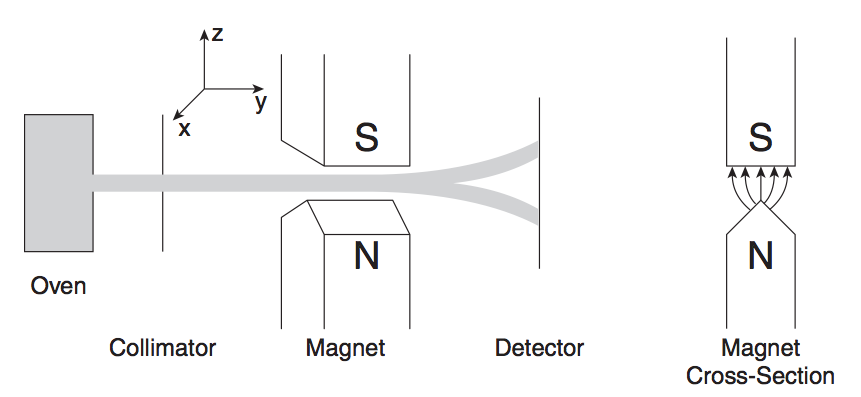
\includegraphics[width=0.8\textwidth]{stern_gerlach.png}
          \caption{Stern-Gerlach experiment to measure the spin component of neutral particles along the $z$-axis. The magnet cross section at right shows the inhomogeneous field used in the experiment.}
       \end{figure}

       This experiment was designed to measure the magnetic dipole moment of a particle (atom). A beam of atoms is passed through a magnetic field gradient and observations are made as to what happens to the trajectory.
       \newline

       So what are the physics in this experiment?

       Potential energy of the magnetic dipole moment $\vec{\mu}$, in external field $\vec{B}$
       \[ E_{magn} = - \vec{\mu} \cdot \vec{B} \]
       The force is negative of the gradient of the potential energy
       \[ \vec{F} = - \vec{\nabla} ( - \vec{\mu} \cdot \vec{B}) \]

       In the Stern Gerlach experiment, the field gradient is in the $z$-direction, so only $\f{dB_z}{dz} \not = 0$, so
       \[ \vec{F} = \mu_z \f{dB_z}{dz} \hat{z} \ \ \ \ \ \mbox{($\hat{z}$ is unit vector in $z$-direction)}\]
       Atoms experience a force in the $z$-direction proportionsl to the $z$-component of magnetic dipole moment $\mu_z$ because we designed an experiment where only $\f{dB_z}{dz} \not = 0$.
       \newline

       What is the classical expectation for silver atoms? (47$e^-$, 47 photons, 60/62 neutrons). Note that
       \[ - \mu_L \mbox{ or } \mu_S \propto \f{1}{m}, \ \ \ \ \mbox{so only consider electrons } (m_p \approx 2000m_e) \]
       and there is only one non-closed (tell electron that contributes to angular momentum), it is in an s-shell $(\vec{L} = 0)$, leaving only instrinsic angular momentum. For silver atoms,
       \[ \vec{\mu} = - g \f{e}{2m_e} \vec{S} \ \ \ \ \mbox{(with $g \approx 2$)} \]
       For a random gas of atoms, $\vec{\mu}$ is in all directions, so $\mu_z$ will have all possible values. So the force will range,
       \[ - \mu \f{dB_z}{dz} \leq |\vec{F}| \leq + \mu \f{dB_z}{dz} \]
       which implies a circular beam spread in the $z$-direction.
       \newline

       It turns out that experimental results reveal that the beam is split into two. This is known as \textbf{space quantization}. This indicates that $S_z$ has two possible values,
       \[ S_z = \pm \f{\hbar}{2} \ \ \ \ \ \ \ \left( \hbar = \f{h}{2\pi} \right) \]
       Splitting is associated with the field gradient $\f{dB_z}{dz}$ since it can change direction and splitting tracks the direction of field gradient. The weird thing here is that \textbf{there is no bias to atom deflection}. There is a 50\% deflection up rate and 50\% deflection down rate. An individual atom is deflected in a probabilistic way. So there is no way of determining precisely what happens to an individual atom.

       \begin{figure}[t!]
          \centering
          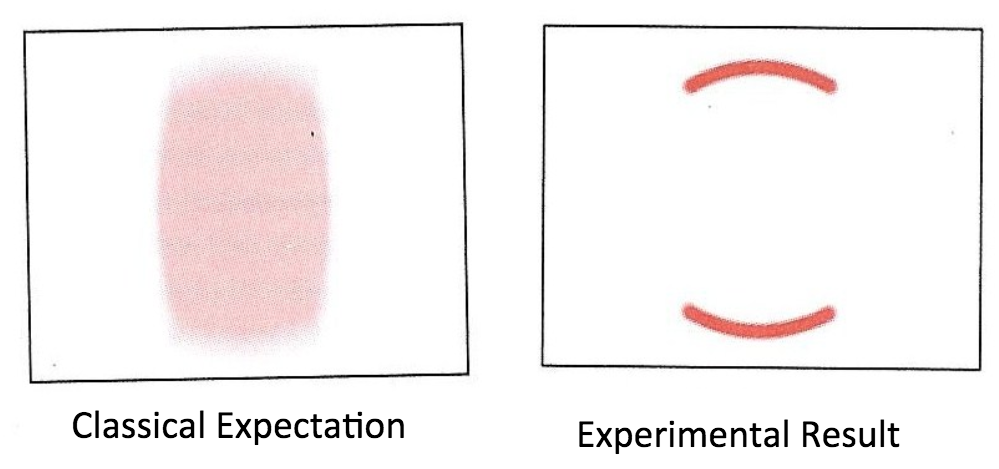
\includegraphics[width=0.5\textwidth]{stern_gerlach_expect.png}
          \caption{Space quantization as it appears in the experimental results of the Stern Gerlach experiment.}
       \end{figure}

       No what we'd like to do is strip down the experiment to the essentisls and introduce language for additional study. First, there are \textbf{two possible outcomes}
       \[ S_z = + \f{\hbar}{2} \ \ \mbox{"spin up"} \ \ \ \ \ \ S_z = - \f{\hbar}{2} \ \ \mbox{"spin down"}  \]
       \begin{defn}[observable]\label{observable}
       The Quantum Mechanics term for the quantity being measured ($S_z$ in this case.)
       \end{defn}
       \begin{defn}[analyser]\label{analyser}
       Stern Gerlach device is some form of an analyser ($x, y, z, \theta, \hat{n}$)
       \end{defn}

       These are being called the essense of quantum mechanics, and there are a number of experiments involved, we're going to analyze each experiment, one by one.

       \subsubsection{Stern-Gerlach Experiment 1}

         \begin{figure}[t!]
            \centering
            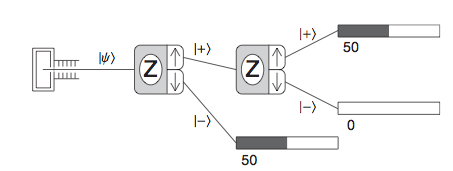
\includegraphics[width=0.5\textwidth]{stern_gerlach_exp1.png}
            \caption{Experiment 1}
         \end{figure}

         In this experiment, no atoms are deflected down at the second analyzer. Also, each analyzer plays a different role; the first analyszer \textbf{prepared} the beam in a specific quantum state ($\ket{+}$) and so it is a \textbf{state preparation device}. The second analyzer \textbf{measures} the prepared beam.

       \subsubsection{Stern-Gerlach Experiment 2}

         \begin{figure}[t!]
            \centering
            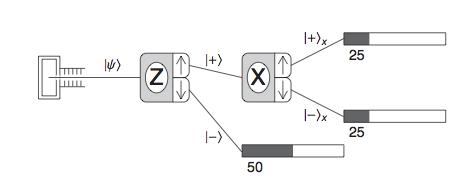
\includegraphics[width=0.5\textwidth]{stern_gerlach_exp2.png}
            \caption{Experiment 2}
         \end{figure}

         The $X$ analyzer has field gradient in the $x$-direction, ($90^{\circ}$ with respect to the $z$-direction). Also, atoms leaving spin-up / spin-down part of the $X$-analyzer have
         \[ S_x = + \f{\hbar}{2} \ \ \ / \ \ S_x = - \f{\hbar}{2} \]
         For input beam $S_z = + \f{\hbar}{2}$ [$\ket{+}$], then 50\% are measured to have $S_x = +\f{\hbar}{2}$. There is the same result for any two different $X$, $Y$, or $Z$ analyser combinations.

       \subsubsection{Stern-Gerlach Experiment 3}

         \begin{figure}[b!]
            \centering
            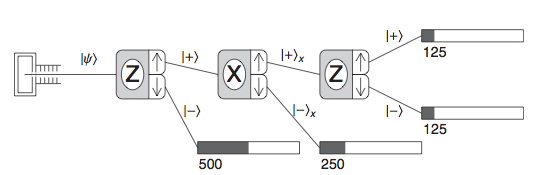
\includegraphics[width=0.5\textwidth]{stern_gerlach_exp3.png}
            \caption{Experiment 3}
         \end{figure}

         Classically, we expect to be able to measure $X$, $Y$, and $Z$ components and figure out the total spin direction.  Experiment 3 shows this is not possible in quantum mechanics, as information is reset or lost when new measurements are made. This is a very generic and key feature of quantum mechanics and comes down to really the statement that \textbf{measurement disturbes the system}. By making a measurement, we change the information of the system. Every time we make a measurement, the system isn't what it was before you made the measurement.
         \newline

         This is a key feature of quantum mechanics. We cannot have simultaneous knowledge of more than one spin component; this is a fundamental incompatability of knowing spin components along two or more directions. We can say that in quantum mechanics, $S_x$, $S_y$, $S_z$ are \textbf{incompatible observables}. More specifically then, the state represented by $\ket{+}_z = \ket{S_z = +\f{\hbar}{2}}$ or $\ket{+}_x = \ket{S_x = + \f{\hbar}{2}}$ but \textbf{not} $\ket{S_z = +\f{\hbar}{2}, S_x = + \f{\hbar}{2}}$.

      \subsubsection{Stern-Gerlach Experiment 4}

         \begin{figure}[t!]
            \centering
            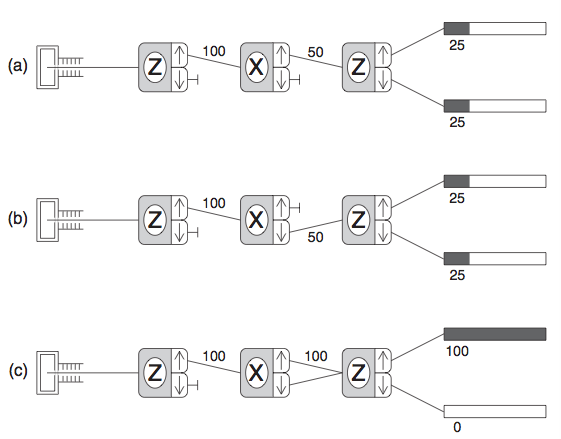
\includegraphics[width=0.5\textwidth]{stern_gerlach_exp4.png}
            \caption{Experiment 4}
         \end{figure}

         The first two demonstrate experiment 3 for both parts of the middle $X$ analyzer independently. The third one gives a surprising result, allowing both parts into the $Z$ analyzer simultaneously then it is as if the middle measurement had not occured. This is reminiscent of interference; adding two outputs results in enhancement in one sector and reduction or cancellation in the other.
         \newline

       In summary,

       \begin{itemize}
         \item Experiment 1: State preparation. If we know the input state and choose an appropriate experiment, we remeasure the state with certainty.
         \item Experiment 2: Probabilistic nature of quantum measurement when the measurement is not matched to the input state.
         \item Experiment 3: Measurement disturbs the system leading to incompatible observables.
         \item Experiment 4: Quantum mechanical interference effects can be observed.
       \end{itemize}

       \subsection{Quantum State Vectors}

         \begin{defn}[Postulate 1]\label{postulate_1}
         We label the input state with a left \textbf{ket}, $(\ket{\Psi}$), and label the output states with $\ket{+}$ for spin up and $\ket{-}$ for spin down.
         \end{defn}

         Thus the ket, $\ket{\Psi}$ is part of a vector space called a \textbf{Hilbert Space}. The dimensionality of the Hilbert Space depends on the \textbf{observable}. For the $S_z$ observable ($z$-component of angular momentum), it has two possible values,
         \[ S_z = \pm \f{\hbar}{2} \]
         Each value is associated with a state vector $\ket{+}$, $\ket{-}$ (note that no subscript will in general mean the $z$-direction, which is just our notation here), so the Hilbert Space is 2D.

         \begin{itemize}
            \item Much like $\hat{x}, \hat{y}, \hat{z}$ vectors span 3D geometric space, the kets $\ket{+}$ and $\ket{-}$ span the 2D Hilbert Space associated with observable $S_z$.
            \item They are \textbf{complete} (only 2 possible outcomes).
            \item They are \textbf{orthogonal}; the result is either spin up or spin down.
            \item They are also \textbf{normalised}; All Quantum state vectors can (or should be) normalized such that $\braket{\Psi}{\Psi} = 1$.
         \end{itemize}

         Orthonormal properties are characterised mathematically as
         \[ \braket{+}{+} = 1 \ \ \ \ \ \ \ \ \braket{+}{-} = 0 \]
         \[ \braket{-}{-} = 1 \ \ \ \ \ \ \ \ \braket{-}{+} = 0 \]

         Completeness ensures that $\ket{+}, \ket{-}$ can be used as a basis to express any general Quantum Mechanical state as a linear combination of them
         \[ \mbox{General State Vector \ \ \ } \ket{\Psi} = a\ket{+} + \ket{-} \mbox{ \ \ \ \ \ with $a, b$ complex scalars}  \]
         The coefficients are inner products, for example consider multiplying on the left by $\ket{+}$,
         \begin{align*}
           \braket{+}{\Psi} & = \braket{+}{\left( a\ket{+}+b\ket{-} \right)} \\
                            & = a\braket{+}{+} + b\braket{+}{-} \\
                            & = a(1) + b(0) \\
                            & = a
         \end{align*}

         Likewise, $\braket{-}{\Psi} = b$. Therfore,
         \[ \ket{\Psi} = \left( \braket{+}{\Psi} \right)\ket{+} + \left( \braket{-}{\Psi} \right) \ket{-} \]
          As an aside, the $\bra{+}$ is the bra to the $\ket{+}$, so together $\braket{+}{+}$ is a bra-ket. $\ddot\smile$.
          \newline

          The dual vector (bra) to the Quantum Mechanical ket $\ket{\Psi}$:
          \begin{align*}
            \bra{\Psi} & = a^*\bra{+} + b^*\bra{-} \\
            \braket{\Psi}{+} & = a^*\braket{+}{+} + b^*\braket{-}{+} = a^*
          \end{align*}
          Hence,
          \[ \braket{\Psi}{+} = a^* = (a)^* = \left( \braket{+}{\Psi} \right)^* = \braket{+}{\Psi}^* \]
          Finally,
          \[ \bra{\Psi} = \left( \braket{\Psi}{+} \right) \bra{+} + \left( \braket{+}{-} \right)\bra{-} \]
          In Quantum Mechanics we require that all kets (vectors) are normalized.

          \begin{exmp}
            Given a general quantum state vector expressed as a linear combination of th ebasis kets for the 2D Hilbert Space associated with the $S_z$ observable:
            \[ \ket{\Psi} = a \ket{+} + b\ket{-} \]
            Derive an expression for the coefficients, $a$ and $b$, which when satisfied ensure that $\ket{\Psi}$ is normalized.
          \end{exmp}

          First we normalize $\ket{\Psi}$, so
          \begin{align*}
             \braket{\Psi}{\Psi} & = 1 \\
             &= \left( a^*\bra{+} + b^*\bra{-} \right)\left( a\ket{+} + b\ket{-} \right) \\
             & =a^*a\braket{+}{+} + a^*b\braket{+}{-} + b^*a\braket{-}{+} + b^*b\braket{-}{-} \\
             & = a^*a + b^*b \\
             & = 1 \mbox{ \ \ \ (requires normalization)} \\
             & = |a|^2 + |b|^2
          \end{align*}
          or since
          \[ a = \braket{+}{\Psi} \ \ \ \ \ a^* = \braket{\Psi}{+} \]
          \[ b = \braket{-}{\Psi} \ \ \ \ \ b^* = \braket{\Psi}{-} \]
          which implies
          \[ \left| \braket{+}{\Psi} \right|^2 + \left| \braket{-}{\Psi} \right|^2 = 1 \]

          \begin{defn}[Postulate 4]\label{postulate_4}
            The probability of obtaining the value $\pm \f{\hbar}{2}$ in a measurement of the observable $S_z$ on a system in the state $\ket{\Psi}$ is
            \[ P_{\pm} = \left| \braket{\pm}{\Psi} \right|^2 \]
            where $\ket{\pm}$ is the basis ket of $S_z$ corresponding to the result $\pm \f{\hbar}{2}$.
          \end{defn}

          \begin{itemize}
            \item[(i)] $\braket{+}{\Psi}$ is the \textbf{Probability Amplitude}, it must be "squared" (multiply by the complex conjugate) to get a probability.
            \item[(ii)] Convention is usually to put order of the inner product as $\braket{\mbox{out}}{\mbox{in}}$ but since
            \[ P = \left| \braket{\mbox{out}}{\mbox{in}}\right|^2  = \braket{\mbox{out}}{\mbox{in}} \braket{\mbox{in}}{\mbox{out}}\]
            it doesn't really matter.
          \end{itemize}
          $\ket{\mbox{in}}$ is the input state, and $\ket{\mbox{out}}$ is the output state, whose probability for measurement we are calculating.

          \begin{exmp}
            A Z-analyzer is used to prepare atoms in the state "spin-up". The spin state if these atoms is then measured using a 2nd Z-analyzer. What is the probability that these atoms are measured as "spin-up" and "spin-down"?
          \end{exmp}
          \[ P = \left| \braket{\mbox{out}}{\mbox{in}} \right|^2 \mbox{ \ \ \ \ \ \nameref{postulate_4}} \]
          The first analyzer prepares the input state to the 2nd analyzer : $\ket{\mbox{in}} = \ket{+}$. The probablilty when $\ket{\mbox{out}} = \ket{+}$ implies that
          \[ P_+ = \left| \braket{+}{+}\right|^2 = 1 \]
          then similary for when $\ket{\mbox{out}} = \ket{-}$ we gey
          \[ P_- = \left| \braket{-}{+}\right|^2 = 0 \]
          This agrees perfectly with our observations for Stern Gerlach Experiment 1.

          \textbf{Quantum State Tomography} is a way of determining the quantum state based on results of measurement and is the name of this method.

          With regards to Stern Gerlach Experiment 2, let's apply this method:
          \newline

          The input state is $\ket{+}$ and we measure $S_x$ with output states $\ket{+}_x$ with probability $\f{1}{2}$ and $\ket{-}_x$ with probability $\f{1}{2}$ (giving a sum probability of 1). Next we formulate mathematically using \nameref{postulate_4} :
          \[ P = \left| \braket{\mbox{out}}{\mbox{in}} \right|^2 \]
          So,
          \begin{align*}
            \ket{\mbox{in}}  = \ket{+} \implies P_{+x} & = \left| {}_x\braket{+}{+} \right|^2 = \f{1}{2} & (1) \\
            P_{-x} & = \left| {}_x\braket{-}{+} \right|^2 = \f{1}{2} & (2) \\
          \end{align*}
          and the result should be the same if $\ket{\mbox{in}} = \ket{-}$ (Experiment 4b)
          \begin{align*}
            \ket{\mbox{in}}  = \ket{-} \implies P_{+x} & = \left| {}_x\braket{+}{-} \right|^2 = \f{1}{2} & (3) \\
            P_{-x} & = \left| {}_x\braket{-}{-} \right|^2 = \f{1}{2} & (4) \\
          \end{align*}
          Since $\ket{+}$ and $\ket{-}$ are basis states that SPAN the 2D Hilbert Space then kets for outputs of other Stern Gerlach measurements can be expressed as linear combinations of them. For example, $S_x$ output states
          \begin{align*}
            \ket{+}_x & = a \ket{+} + b\ket{-} \\
            \ket{-}_x & = c \ket{+} + d\ket{-}
          \end{align*}
          for $a,b,c,d \in \C$. Now,
          \begin{align*}
            P_{+x} & = \left| {}_x\braket{+}{+} \right|^2 & = \left| \left( a^*\bra{+} + b^*\bra{-} \right)\ket{+} \right|^2 \\
            & = \left|  a^*\braket{+}{+} + b^*\bra{-}{+} \right|^2 \\
            & = |a|^2 \\
            & = \f{1}{2} \mbox{ \ \ \ \ \ (from experiment)}
          \end{align*}
          Similary we can use (2), (3), and (4) to show that $|b|^2 = |c|^2 = |d|^2 = \f{1}{2}$.
          \newline

          The coefficients $a,b,c,d$ are complex numbers implying that the amplitude of the phase is
          \[ re^{i\theta} \]
          \begin{note}
            The overall phase (global phase) of a quantum state vector is not physically meaningful - this means it doesn't affect the computation of probabilities (Assignment 3).
          \end{note}

          Only the relative phase between components of a ket (vector) is important, that is between $a$ and $b$ or $c$ and $d$. This means that we chose one component to be real ($\theta = 0$) and one complex ($\theta \not = 0$).
          \newline

          Say $a = r_1e^{i\theta_1}$ and $b = r_2e^{i\theta_2}$, then only $\theta_2 - \theta_1$ matters for quantum mechanics so we rotate the vectors to make one real. \newline

          This means we can solve for $a$, $b$, $c$, and $d$ in the following way
          \begin{align*}
            \ket{+}_x & = \f{1}{\sqrt{2}}\ket{+} + \f{1}{\sqrt{2}}e^{i\alpha}\ket{-} \\
            \ket{-}_x & = \f{1}{\sqrt{2}}\ket{+} + \f{1}{\sqrt{2}}e^{i\beta}\ket{-}
          \end{align*}

          We can check,

          \[ P_{+x} = \left| \braket{\mbox{out}}{\mbox{in}} \right|^2 = \left| \left( \f{1}{\sqrt{2}}\ket{+} + \f{1}{\sqrt{2}}e^{i\alpha}\ket{-} \right) \ket{+} \right|^2 = \f{1}{2}\]


%%%%%%%%%%%%%%%%%%%%%%%%%%%%%%%%%%%%%%%%%%%%%%%%%%%%%%%%%%%%%%%%%%%%%%%%%%%%%%%%%%%%%%%%%

   \section{Tutorials}

     \subsection{Tutorial 1}

     \begin{itemize}
       \item[1.] Given two vectors
       \[ \va = \mtx{1 \\ 2 \\ 4}, \ \ \ \  \vb = \mtx{6 \\ 4 \\ 1} \]
       \begin{itemize}
         \item[(a)] Compute the inner product $\va^T\vb$ \\
           \[ 1\cdot6 + 2\cdot4 + 4\cdot 1 = 12 \]
         \item[(b)] Compute the outer product $\va\vb^T$
           \[ 6 \cdot 1 + 4\cdot2 + 1\cdot4 = 12 \]
       \end{itemize}
       \item[2.] Given two matrices
       \[ A = \mtx{1 & 9 \\ 4 & 3}, \ \ \ \ B = \mtx{0 & 2 \\ 5 & 6} \]
       \begin{itemize}
         \item[(a)] Compute the product $AB$
           \[ \mtx{1\cdot0 + 9\cdot5 & 1 \cdot2 + 9\cdot 6 \\ 4 \cdot 0 + 3 \cdot 5 & 4 \cdot 2 + 3 \cdot 6} = \mtx{45 & 56 \\ 15 & 20}\]
         \item[(b)] Do these matrices commute? \\
           Let's check
           \[ \mtx{ 0 \cdot 1 + 2 \cdot 4 & 0 \cdot 9 + 2 \cdot 3 \\ 5\cdot1 + 6 \cdot 4 &  5 \cdot 9 + 6\cdot 3 } = \mtx{8 & 6 \\ 29 & 63} \]
           No.
       \end{itemize}
       \item[3.] Given the matrix
       \[ C = \mtx{7 & 2 \\ 2 & 4} \]
       \begin{itemize}
         \item[(a)] Compute the eigenvalues of $C$
           The characteristic polynomial is
           \[ C(\lambda) = \det{(C - \lambda I)} = \det \mtx{7 - \lambda & 2 \\ 2 & 4 - \lambda} = (7-\lambda)(4-\lambda) - 4  = 24 -11\lambda + \lambda^2 \implies \lambda = 8, 3 \]
         \item[(b)] Compute the eigenvectors of $C$
           \[ C - 8I = \mtx{-1 & 2 \\ 2 & -4 } \equiv \mtx{-1 & 2 \\ 0 & 0} \implies \vv = t\mtx{2 \\ 1} \ \ \ \ s, t \in \R\]
           \[ C - 3I = \mtx{4 & 2 \\ 2 & 1 } \equiv \mtx{0 & 0 \\ 2 & 1} \implies \vv = t\mtx{-1 \\ 2} \ \ \ \ s, t \in \R\]
         \item[(c)] Are the eigenvectors orthogonal?
         \[ \mbox{Yes.} \]
         \item[(d)] Normalize the eigenvectors.
         \[ \mtx{\f{2}{\sqrt{5}} \\ \f{1}{\sqrt{5}}}, \mtx{\f{-1}{\sqrt{5}} \\ \f{2}{\sqrt{5}}} \]
       \end{itemize}
       \item[4.] Given the complex number
       \[ z = 3 + 3i \]
       \begin{itemize}
         \item[(a)] Compute the complex conjugate of $z$ (denoted $\bar{z}$)
            \[ \bar{z} = 3 - 3i \]
         \item[(b)] Compute the norm of $z$ (denoted $|z|$)
            \[ |z| = \sqrt{z\cdot \bar{z}} = \sqrt{18} \]
         \item[(c)] Express $z$ as $z = re^{i\theta}$.
            \[ z = (\sqrt{18})e^{i\arctan\left( \f{3}{3} \right)} = \sqrt{18}e^{\f{\pi i}{2}} \]
         \item[(d)] Express $z$ as $z = r(cos\theta + i\sin\theta)$
             \[ z = \sqrt{18}\left(\cos \f{\pi}{2} + i\sin \f{\pi}{2}\right) \]
       \end{itemize}
     \end{itemize}

     \subsection{Tutorial 2}

      Tutorial 2 concerns coin flipping, the SPINS program, and connections to Quantum Theory. We played games.

     \subsection{Tutorial 3}

      We are given a matrix $M_2 = \mtx{1 & 0 \\ 0 & -1}$, so first we find the eigenvalues:
      \[ (1-\lambda)(-1 - \lambda) = 0 \implies \lambda = \pm 1 \]
      Then for $\lambda_1 = 1$ we get
      \[ \mtx{0\\0} = \mtx{0 & 0 \\ 0 & -2}\mtx{x_1 \\ x_2} \implies \vv_1 = \mtx{1 \\ 0} \]
      and $\lambda_2 = -1$ which corresponds to $\vv_2 = \mtx{0 \\ 1}$. Now we want to determine if this matrix is a reflection and if so on what line; well actually this is pretty straightforward because you can see that for any vector, $M_2\mtx{x_1\\x_2} = \mtx{x_1\\-x_2}$ which means it is a vertical reflection (over the $x$-axis).
      \newline

      Also a little bit on Group Theory.

  \end{document}
